\chapter{Evaluierung}\label{kap:eval}

Bevor die Ergebnisse der trainierten Modell diskutiert 
werden, behandelt dieses Kapitel zunächst einige der für die 
Objekterkennung üblicherweiser verwendeten Metriken zur Messung
der Genauigkeit. 


Anschließend werden die Modell in \ref{sec:model_vergleich}
miteinander verglichen und in \ref{sec:optimierung_faster_rcnn}
optimierungsverfahren für das Faster R-CNN Model ausgewertet.


\section{Evaluierungs Metriken}\label{sec:metricen}

\subsection*{Mean Average Precision (mAP)}

Als Metrik für die Genauigkeit eines Object Detection Models 
dient die \textit{Mean Average Precision (mAP)}, welche 
sowohl Klassifizierung als auch Lokalisierung mit einbezieht 
und sich aus folgenden Werten berechenn lässt.


\begin{itemize}
  \item \textit{True Positive (TP)}: 
  \item \textit{True Negative (TN)}: 
  \item \textit{False Positive (FP)}: 
  \item \textit{False Negative (FN)}: 
\end{itemize}

Zur bestimmung dieser Werte wird die \textit{Intersection over unioun}
verwendet, welche Überlappungsgrad der gelabelten (Ground Truth) und der
geschätzete Boundig Box zu dem Gesammtbereich beider Boxen darstellt 

Beträgt dieser mehr als ein Bestimmter Threshhold, häufig 50\%
gilt die Schätzung als \textit{True Positive}, andernfalls als 
\textit{False Positive}. 


% für confusion matrix
\newcommand\MyBox[2]{
  \fbox{\lower0.75cm
    \vbox to 1.7cm{\vfil
      \hbox to 1.7cm{\hfil\parbox{1.4cm}{#1\\#2}\hfil}
      \vfil}%
  }%
}
\noindent
\renewcommand\arraystretch{1.5}
\setlength\tabcolsep{0pt}

\begin{minipage}{\textwidth}
    \begin{minipage}[b]{0.49\textwidth}
      \centering
      \def\svgwidth{0.8\textwidth}
      \input{Bilder/IoU_formula.pdf_tex}
      \captionof{figure}{Intersection over Union}
      \label{fig:iou}
  \end{minipage}
    \hfill
    \begin{minipage}[b]{0.49\textwidth}
      \centering
      \begin{tabular}{c >{\bfseries}r @{\hspace{0.7em}}c @{\hspace{0.4em}}c @{\hspace{0.7em}}l}
        \multirow{10}{*}{\rotatebox{90}{\parbox{2.5cm}{\bfseries\centering Tatsächlicher Wert}}} & 
          & \multicolumn{2}{c}{\bfseries Geschätzter Wert} & \\
        & & \bfseries p & \bfseries n & \bfseries\\
        & p$'$ & \MyBox{True}{Positive} & \MyBox{False}{Negative}\\[2.4em]
        & n$'$ & \MyBox{False}{Positive} & \MyBox{True}{Negative} \\
      \end{tabular}
        \captionof{figure}{Confusion Matrix}
    \end{minipage}
\end{minipage}


\vspace{1cm}
    
Daraus lassen sich dann Precision und Recall berechnen. 

\textit{Recall}
welcher angibt wie 
viele Objekte das Modell gefunden hat
\begin{equation}
  Recall = \frac{TP}{TP + FN}
\end{equation}
TP + FN allen Objekten im Bild entspricht, somit also das 
Verhälltnis der Gefunden zu allen Objekten im Bild


\textit{Precision}
die angibt mit welcher Genauigkeit die Objekte gefunden wurden
\begin{equation}
  Precision = \frac{TP}{TP + FP}
\end{equation}
also die richtig 
geschätzen durch alle gemachten schätzunge und gibt somit die 
genauigkeit mit der das Model die Objekte findet an.


\textit{Average Precision}
\begin{equation}
  Average Precision = \frac{1}{N}\sum(Precision(Recall))
\end{equation}

Daraus kann nun die durchschnittliche Precision für alle Recall 
Werte bestimmt werden, welche als \textit{Average Precision}
bezeichnet wird und die Genauigkeit des Models bezogen auf 
eine bestimmte Klasse angibt

\textit{mean Average Precision}
Für alle Klassen gemittel 
erhält man die mittlere durchschnittliche Precision (mAP)



\subsection*{Fehlerfunktion (Loss)}
Die Fehlerfunktion setzet sich aus einem Lokalisierungs und einem 
Klassifizierungsfehler zusammen. 
Die Lokalisierung erfolgt über eine Lineare Regression zur 
Annäherung der Bounding Boxes and die richtigen Koordinaten.\\

Bei Faster R-CNN werden diese beiden Loss Werte dann sowohl für 
RPN(1st stage) als auch für classifier(2nd stage) also 
insgesammt 4 loss werte verwendet.



%----------------- SECTION: validtaion ---------------------
\section{Vergleich der Modelle}\label{sec:model_vergleich}
In diesem Abschnitt werden die beiden für das Training verwendeten
Objec Detection Architekturen Single Shot Detector (SSD)
und Faster R-CNN miteinander verglichen.



\subsection{Evaluierung/Validierung}

Die Evaluierungsergebnisse beziehen sich auf das 
Testsets aus dem Open Images Datensatz.
\\
SSD wurd mit Batchsize=12 75k durchläufe trainiert.\\
Faster R-CNN mit Batchsize=1 für 200k durchläufe.(1 weil dynamische input size)\\
eine epoche sind (teps mal batchsize)/samples
\\
\begin{table}[H]
  \centering
  \begin{tabular}{m{0.25\textwidth}m{0.2\textwidth}|m{0.15\textwidth}<{\centering}m{0.15\textwidth}<{\centering}}
  \hline
  Model                                                              & Optimierung                                                                   & mAP                                                        & Loss                                                       \\ \hline\hline
  SSD + MobilenetV2                                                  & \begin{tabular}[c]{@{}l@{}}Ohne\\ Augmentierung\end{tabular}                  & \begin{tabular}[c]{@{}l@{}}0,62\\ 0,61\end{tabular}        & \begin{tabular}[c]{@{}l@{}}3,56\\ 3,50\end{tabular}        \\ \hline
  SSD + InceptionV2                                                  & \begin{tabular}[c]{@{}l@{}}Ohne\\ Augmentierung\end{tabular}                  & \begin{tabular}[c]{@{}l@{}}0,65\\ 0,62\end{tabular}        & \begin{tabular}[c]{@{}l@{}}3,86\\ 3,71\end{tabular}        \\ \hline
  \begin{tabular}[c]{@{}l@{}}Faster R-CN\\ +InceptionV2\end{tabular} & \begin{tabular}[c]{@{}l@{}}Ohne\\ Augmentierung\\ Early Stopping\end{tabular} & \begin{tabular}[c]{@{}l@{}}0,67\\ 0,69\\ 0,67\end{tabular} & \begin{tabular}[c]{@{}l@{}}0,82\\ 0,67\\ 0,69\end{tabular} \\ \hline
  \end{tabular}
\end{table}

Man kann erkennen das der Feler (Loss) durch Augmentierung etwas 
veringert wurde.
Insbesondere beim Faster R-CNN, welches aufgrund der 
höheren komplexität, schneller zur überanpassung neigt.\\
Der Verlauf des Trainings ließ sich mihilfe des Evaluierungstools Tensorboard
Visualisieren, Plots für die drei Konfigurationen des Faster R-CNN sind in 
Abbildung \ref{plot:mAP} und \ref{plot:loss} dargestellt.
\vspace{0.5cm}

\begin{figure}[htb]
\begin{minipage}{0.5\textwidth}
  \centering
  \label{plot:mAP}
  \def\svgwidth{0.9\textwidth}
  \input{Bilder/plots/overfitting_kein_early_aug_mAP.pdf_tex}
  \captionof{figure}{mAP}
\end{minipage}
\begin{minipage}{0.5\textwidth}
  \centering
  \label{plot:Loss}
  \def\svgwidth{0.9\textwidth}
  \input{Bilder/plots/overfitting_kein_early_aug_loss.pdf_tex}
  \captionof{figure}{Loss}
\end{minipage}
\end{figure}

% Legende: Overfitting
\begin{table}[htb]
  \centering
  \begin{tabular}{m{0.1\textwidth}<{\centering}m{0.2\textwidth}<{\centering}m{0.2\textwidth}<{\centering}}
    $\color[HTML]{FF7043}\medbullet$  Ohne & $\color[HTML]{0077BB}\medbullet$  Early Stopping & $\color[HTML]{CC3311}\medbullet$  Augmentierung
  \end{tabular}    
\end{table}

% colors
% orange: FF7043
% blue  : 0077BB
% red   : CC3311



hier die zwi techniken zur vermeidung von overfitting: augmentierung
und Loss gegenübergestellt. Augmentierung erzielt bessere ergebnisse, 
da durch vorzeitiges stoppen des trainings auch keine weitere verbesserung
bezüglich mAP mehr stattfinden konnte.

% weitere Beobachtung: wenn eval für anderes Datenset 
% angewendet wird ist auch der Loss des Augmentierten 
% Datensets besser.



%----------------- SECTION: Test Inferenz ---------------------
\subsection{Test Inferenz}\label{sec:test_inferenz}

Um eine bessere Vorstellung davon zu bekommen wie sich die 
unterschiedlichen Ergebnisse in mAP und Loss in der Anwendung 
tatsächlich bemerkbar machen, wurde die Inferenz der drei modelle 
für verschiedene Test Bilder durchgeführt.

Dafür wurden die Modelle in die für OpenVino benötigte Intermediate
Representation umgewandelt um dann mihilfe eines Python 
Scripts in die InferenceEngine geladen zu werden.

Mithilfe dieses Scripts konnten nun die Inferenz für 
folgende Testszenarien:

\begin{itemize}
  \item inferenz auf Test Set \textit{OpeImages}
  \item inferenz auf \textit{The iWildCam 2019 Dataset}\cite{beery2019iwildcam}
  \item inferenz auf eigene Bilder
\end{itemize}


\subsubsection{Test Set (OpenImages)}
Sowohl SSD als auch Faster R-CNN erkennen das meiste, da gr 
ähnlichkeit zu Trainingssatz.

Wenn jedoch mehrere Tiere im Bild sind, diese weiter weg oder schlechtere
Bildqualität, erkennt Faster R-CNN besser. Abb \ref{fig:faster_rcnn}
\\[1cm]
\begin{minipage}{0.5\textwidth}
  \centering
  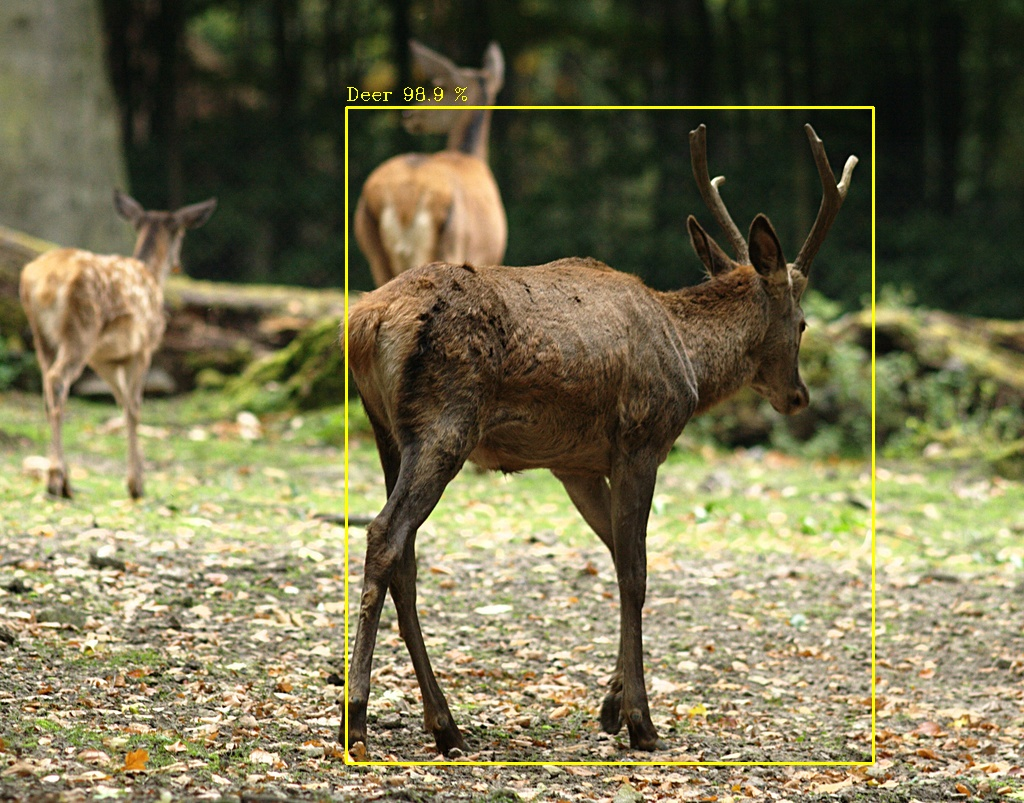
\includegraphics[width=0.9\textwidth]{model_compare_test__ssd_inception_v2.jpg}
  \captionof{figure}{SSD}
  \label{fig:ssd}
\end{minipage}
\begin{minipage}{0.5\textwidth}
  \centering
  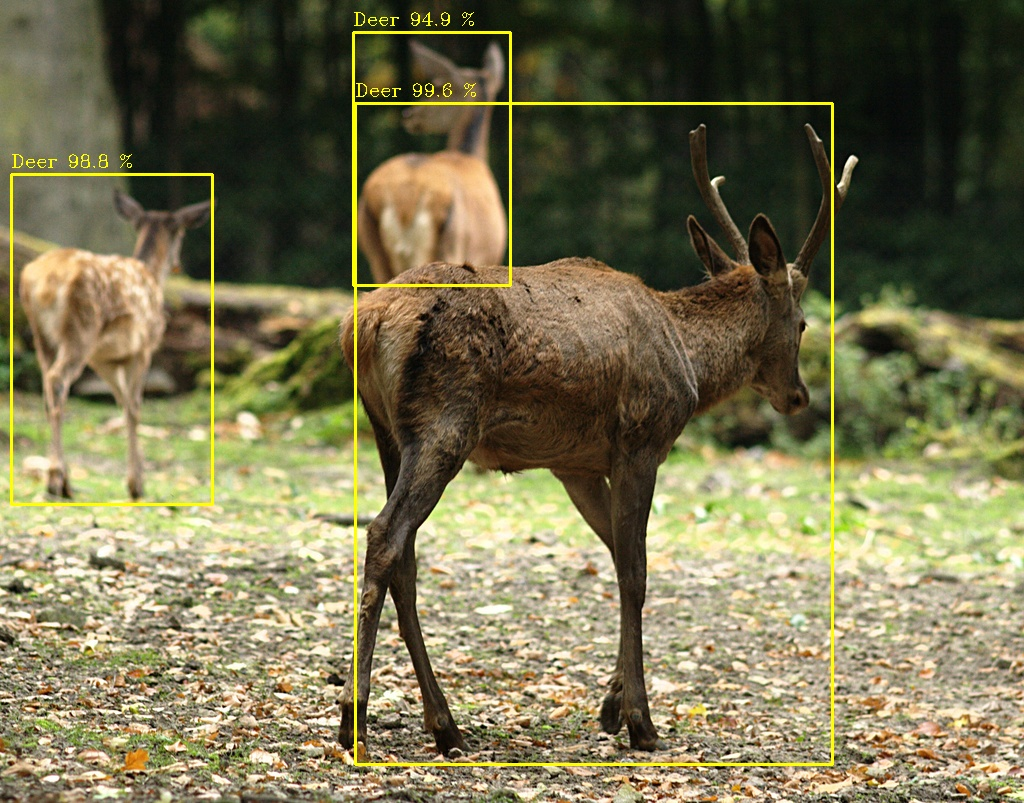
\includegraphics[width=0.9\textwidth]{model_compare_test__faster_rcnn_inception_v2_early_stopping.jpg}
  \captionof{figure}{Faster R-CNN}
  \label{fig:faster_rcnn}
\end{minipage}


\subsubsection{Eigene Aufnahmen}

\begin{minipage}{0.5\textwidth}
  \centering
  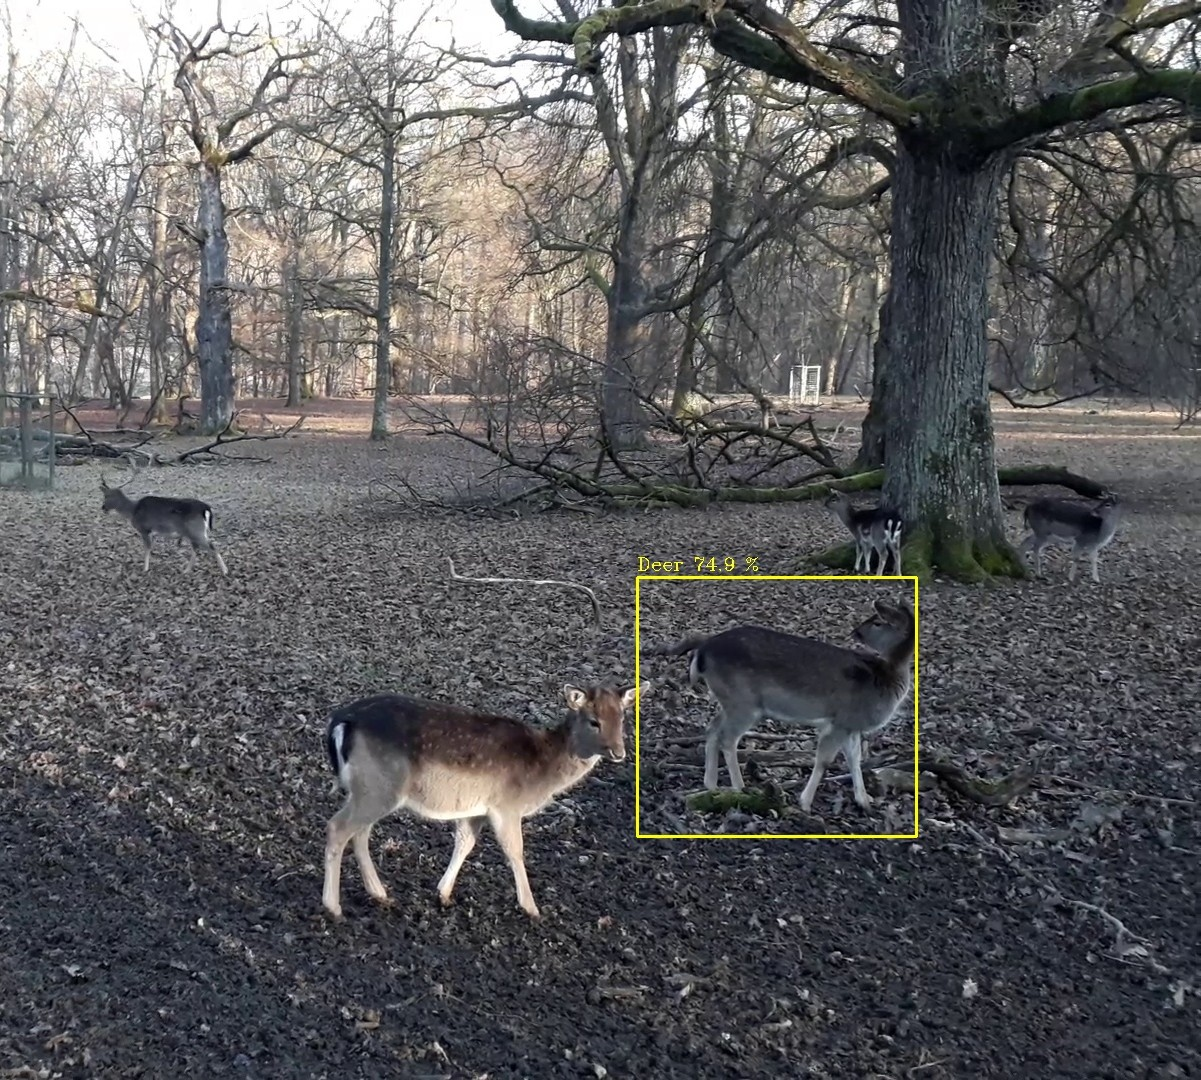
\includegraphics[width=0.9\textwidth]{model_compare_handy_ssd_mobilenet_v2.jpg}
  \captionof{figure}{SSD Mobilnet}
  \label{}
\end{minipage}
\begin{minipage}{0.5\textwidth}
  \centering
  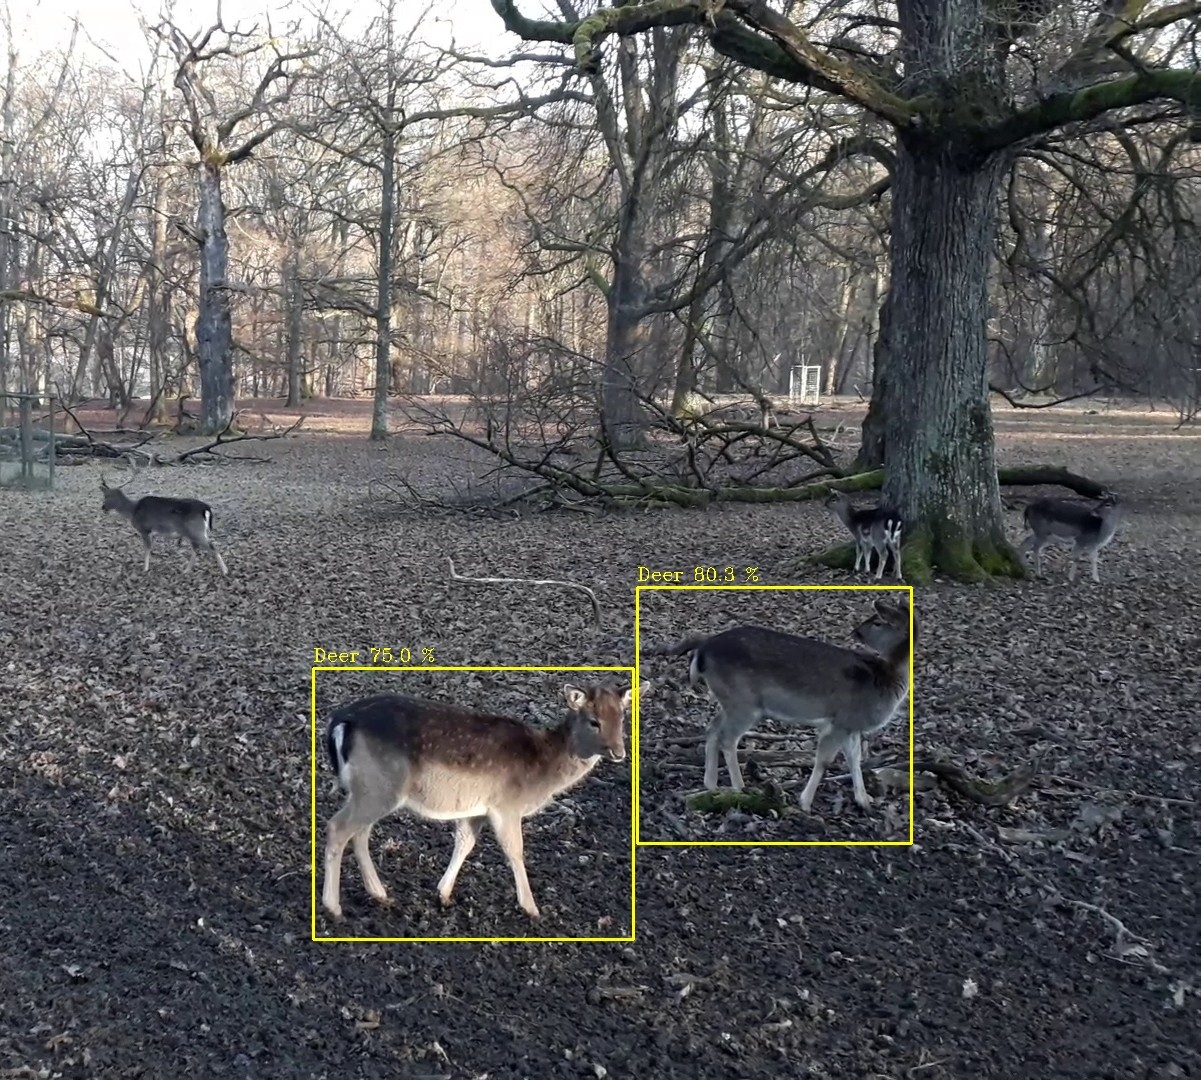
\includegraphics[width=0.9\textwidth]{model_compare_handy_ssd_inception_v2.jpg}
  \captionof{figure}{SSD Inception}
  \label{}
\end{minipage}
\\[1cm]
\begin{minipage}{0.5\textwidth}
  \centering
  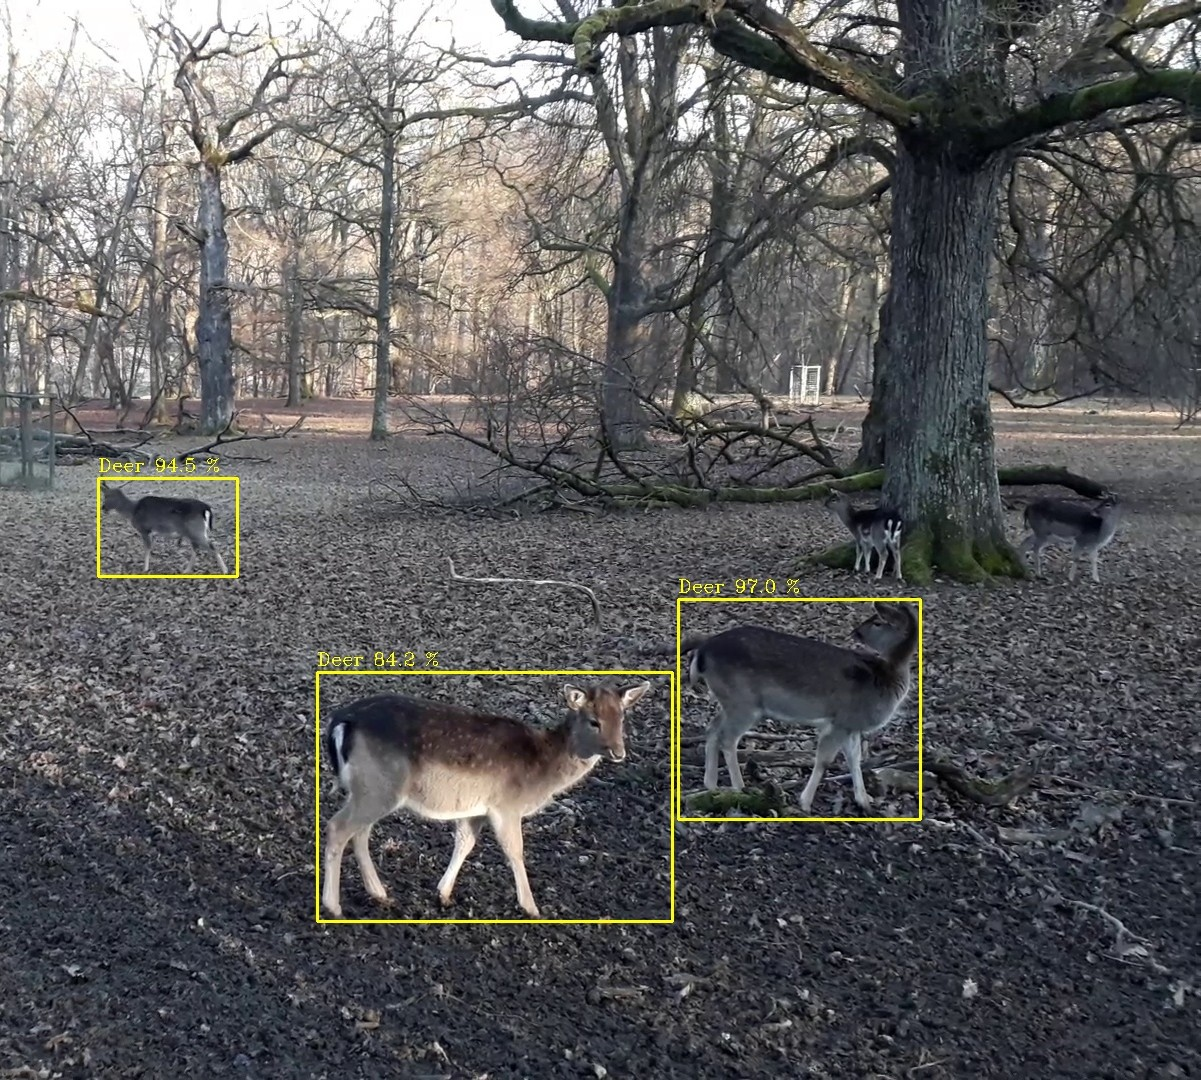
\includegraphics[width=0.9\textwidth]{model_compare_handy_faster_rcnn_inception_v2_early_stopping_ohne_aug.jpg}
  \captionof{figure}{Faster R-CNN + Early Stopping}
  \label{}
\end{minipage}
\begin{minipage}{0.5\textwidth}
  \centering
  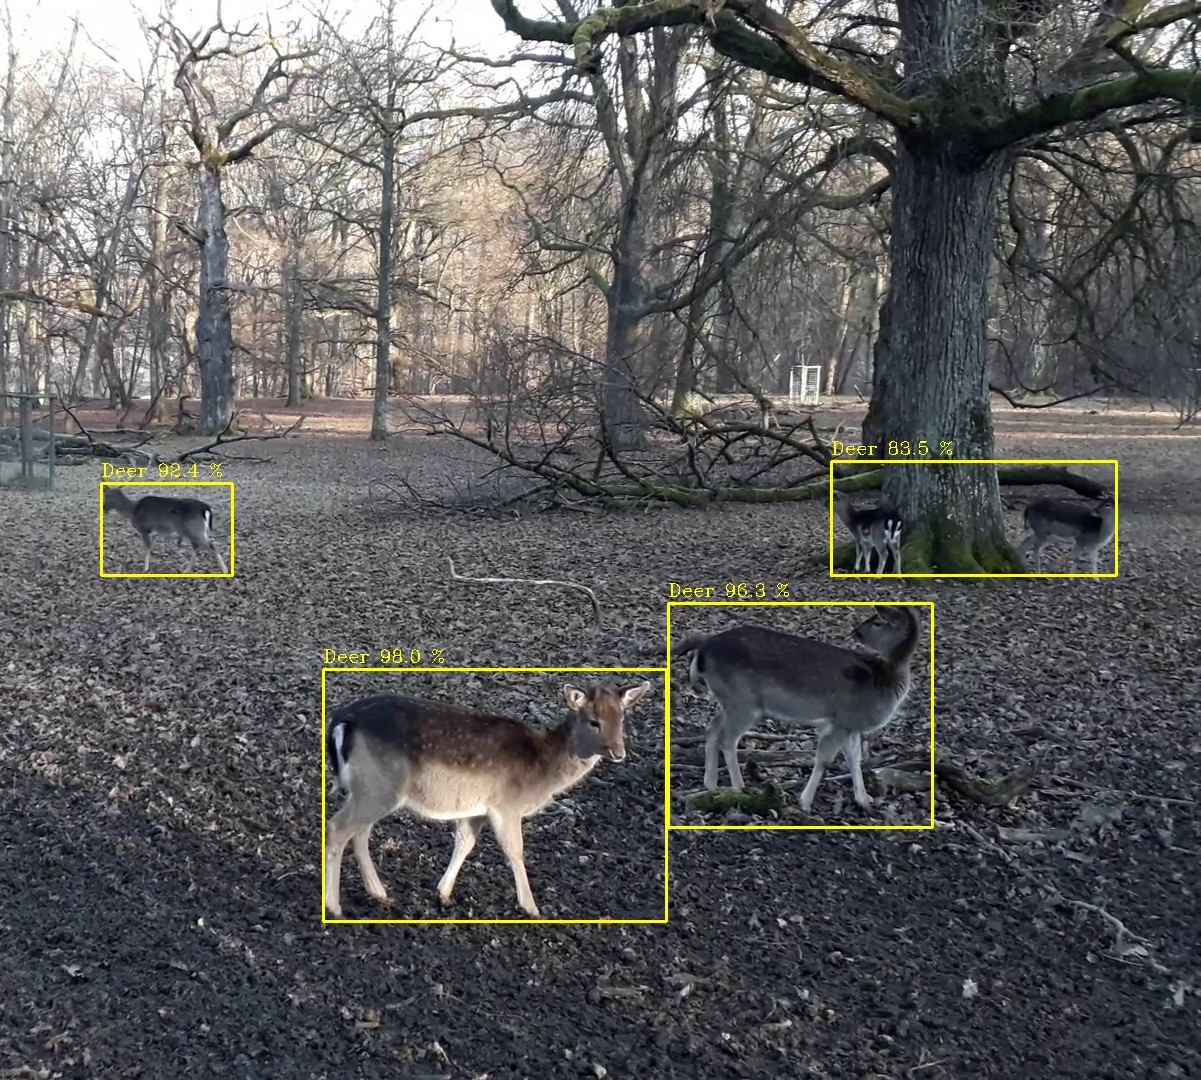
\includegraphics[width=0.9\textwidth]{model_compare_handy_faster_rcnn_inception_v2_early_stopping.jpg}
  \captionof{figure}{Faster R-CNN + Aug}
  \label{}
\end{minipage}


\subsubsection{iWildCam}

Aufnahmen von ... enthällt viele schlecht beleuchtete nacht Aufnahmen 
mit Infrarot Kamera, also ähnlich dem gewünschten Anwendungsfall.
Auch hier erkennt das Faster R-CNN am beste, jedoch 
schneiden hier alle schlecht ab.

Daher wurde, wie im nächsten Abschnitt beschrieben, versuch
das Faster R-CNN noch weiter zu optimieren.


%----------------- SECTION: optimierung ---------------------
\section{Optimierungen: Faster R-CNN}\label{sec:optimierung_faster_rcnn}


Als Ausgangslage zur verbesserung der Ergebnisse diente 
nun das Faster R-CNN mit augmentiertem Datensatz, welches 
im vorherigen Abschnitt die besten Resultate erzielte.

Auch hier werden zunächst die Ergebnisse zunächst wieder 
anhand der Eval Metriken für den Validierungsdatensatz mithilfe Tensorboard 
dargestellt und anschließend mit Testdatensatz sowie weitere testinferez 
durchgeführt.




\subsection{Verschiedene Augmentierungen}

Der erste Anstz war es dieses mit variierendem Augmentierungsgrad 
für insgesamt mehr Trainingsdurchläufe (500 statt 200) zu 
trainieren.

Im vorherigen Abschnitt wurde für die Augmentierung der 
Daten je Bild zufällig aus einer auswahl eine geometrische und eine 
Pixelbezogene augmentierungstechnik angewendet, sodass für jede Klass 
3000 Samples genriert wurden.

Als vairation wurde hier nun einmal die gleiche Augmentierungsstrategie 
für 4000 samples und einmal nur einer Augmentierung pro Bild für 
3000 Samples angewendet.

Die Trainingskurven aus Tensorboard sind für mAP und Loss sind in den
Plots \ref{plot:map_diff_aug} und \ref{plot:loss_diff_aug} dargestellt.
\vspace{1cm}

\begin{minipage}{0.5\textwidth}
  \centering
  \label{plot:map_diff_aug}
  \def\svgwidth{0.9\textwidth}
  \input{Bilder/plots/diff_aug_map.pdf_tex}
  \captionof{figure}{mAP}
\end{minipage}
\begin{minipage}{0.5\textwidth}
  \centering
  \label{plot:loss_diff_aug}
  \def\svgwidth{0.9\textwidth}
  \input{Bilder/plots/diff_aug_loss.pdf_tex}
  \captionof{figure}{Loss}
\end{minipage}

% Legende
\begin{table}[htb]
  \centering
  \begin{tabular}{m{0.1\textwidth}<{\centering}m{0.2\textwidth}<{\centering}m{0.2\textwidth}<{\centering}}
    $\color[HTML]{CC3311}\medbullet$  1 je bild & $\color[HTML]{FF7043}\medbullet$  3000 samples & $\color[HTML]{0077BB}\medbullet$  4000 samples
  \end{tabular}    
\end{table}

Es ist zu erkennen, das sich durch stärkere augmentierung der Trainingsdaten
der Loss reduzieren lässt, dadurch jedoch auch der mAP abnimmt.

% colors
% orange: FF7043
% blue  : 0077BB
% red   : CC3311



\subsection{weitere Regularisierungen}

Um das trotz Augmentierung zu stande kommende Overfitting zu 
vermeiden, wurden nun zusätzlich die L2 Regularisierung angewendet.
Diese soll wie in den Grundlagen (\ref{subsec:validation}) beschrieben, 
durch anfügen der aufsummierten Geweichte an die Loss Funktion, 
die Überanpassugne eindämmen.

In der Konfigurationsdatei des Fater R-CNN kann dies durch setzten des 
bestimmten Parameters für sowohl die erste Stufe, das RPN (Region Proposal Network)
als auch für die 2. Stufe, das Klassifizierungsnetz seperat gesetz werden.


Ebenso lassen sich die beiden Losskurven, aus denen sich der gesammt 
Loss zusammensetz, seperat anzeigen, wie in Plot \ref{plot:aug_l2_classifier_loss}
und \ref{plot:aug_l2_rpn_loss} zu erkennen ist.

Dadurch ließ sich feststellen, dass Overfitting nur beim Loss des RPNs 
stattfindet, weshalb der L2 Parameter auch nur für die erste Stufe 
das RPN engestellt wurde. Dabei wurde der Fa $\lambda = 0.001$ verwendet.

Schaut man nun wieder die beiden Losskurven an, zeigt sich deutlich der 
Effekt, den die L2 Regularisierung auf den RPN Loss hat, was sich dann 
auch im Gesammtloss durch eine leichte verbesserung bemerkbar machte.

\vspace{1cm}


\begin{minipage}{0.5\textwidth}
  \centering
  \def\svgwidth{0.9\textwidth}
  \input{Bilder/plots/aug_l2_mAP.pdf_tex}
  \captionof{figure}{mAP}
  \label{plot:aug_l2_mAP}
\end{minipage}
\begin{minipage}{0.5\textwidth}
  \centering
  \def\svgwidth{0.9\textwidth}
  \input{Bilder/plots/aug_l2_total_loss.pdf_tex}
  \captionof{figure}{Total Loss}
  \label{plot:aug_l2_total_loss}
\end{minipage}
\\[1cm]
\begin{minipage}{0.5\textwidth}
  \centering
  \def\svgwidth{0.9\textwidth}
  \input{Bilder/plots/aug_l2_classifier_loss.pdf_tex}
  \captionof{figure}{Classifier Loss}
  \label{plot:aug_l2_classifier_loss}
\end{minipage}
\begin{minipage}{0.5\textwidth}
  \centering
  \def\svgwidth{0.9\textwidth}
  \input{Bilder/plots/aug_l2_rpn_loss.pdf_tex}
  \captionof{figure}{RPN Loss}
  \label{plot:aug_l2_rpn_loss}
\end{minipage}
\begin{table}[htb]
  \centering
  \begin{tabular}{m{0.3\textwidth}<{\centering}m{0.4\textwidth}<{\centering}}
    $\color[HTML]{CC3311}\medbullet$  nur Augmentierung & $\color[HTML]{0077BB}\medbullet$  Augmentierung+L2 Regulierung
  \end{tabular}    
\end{table}

\vspace{1cm}

Dies wurde ebenso auf das Training mit weniger stark augmentiertem Datensatz
angewendet. Weitere Einstellungen waren $\lambda = 0.002$ und das 
ebenfalls in \ref{subsec:validation} beschriebene Dropout.
Die ergebnisse sind nocheinmal zusammefassend in Tabelle ... dargestellt.


\begin{table}[htb]
  \centering
  \label{table:reg}
  \begin{tabular}{m{0.2\textwidth}|m{0.2\textwidth}<{\centering}m{0.2\textwidth}<{\centering}m{0.2\textwidth}<{\centering}}
  \hline
  \textgreater 400k & mAP  & Loss (Gesammt) & Loss (RPN) \\ \hline\hline
  Augmentierung     & 0,7  & 0,74           &  0,12          \\
  +Dropout          & 0,7  & 0,73           &            \\
  +L2 Reg (0.01)    & 0,7  & 0,69           &            \\
  +L2 Reg (0.02)    & 0,69 & 0,7            &            \\ \hline
  \end{tabular}
  \caption{Regularisierungen}
\end{table}


\subsection{Test Inferenz}

Auch hier wurde nun wieder zur besseren Auswertung der Ergebnisse die 
Inferez Testweise auf die drei Datensätze Test Set des trainierten Open Images
Datensatzes, eigen Aufnahmen, sowie des \textit{iWildCam} Datensatzes durchgeführt.

\begin{minipage}{0.333\textwidth}
  \centering
  \label{}
  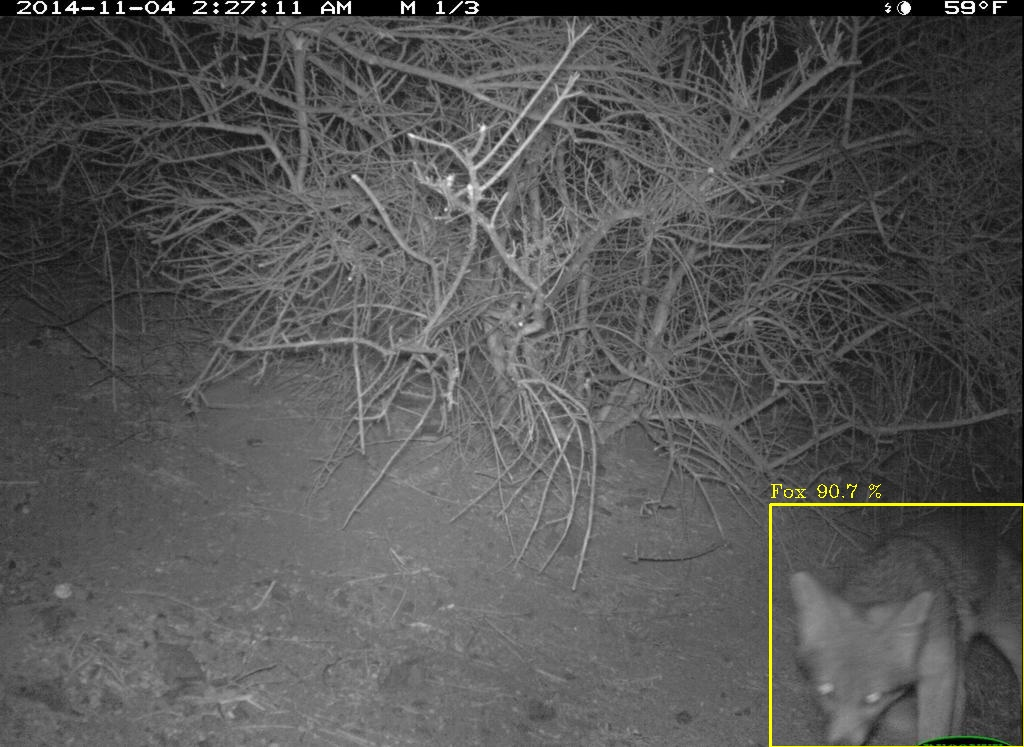
\includegraphics[width=\textwidth]{infer_images/iWildCam/fox/cut/59df5ee1-23d2-11e8-a6a3-ec086b02610b_faster_rcnn_inception_v2_3000.jpg}
  \captionof{figure}{3000 Samples}
\end{minipage}
\begin{minipage}{0.333\textwidth}
  \centering
  \label{}
  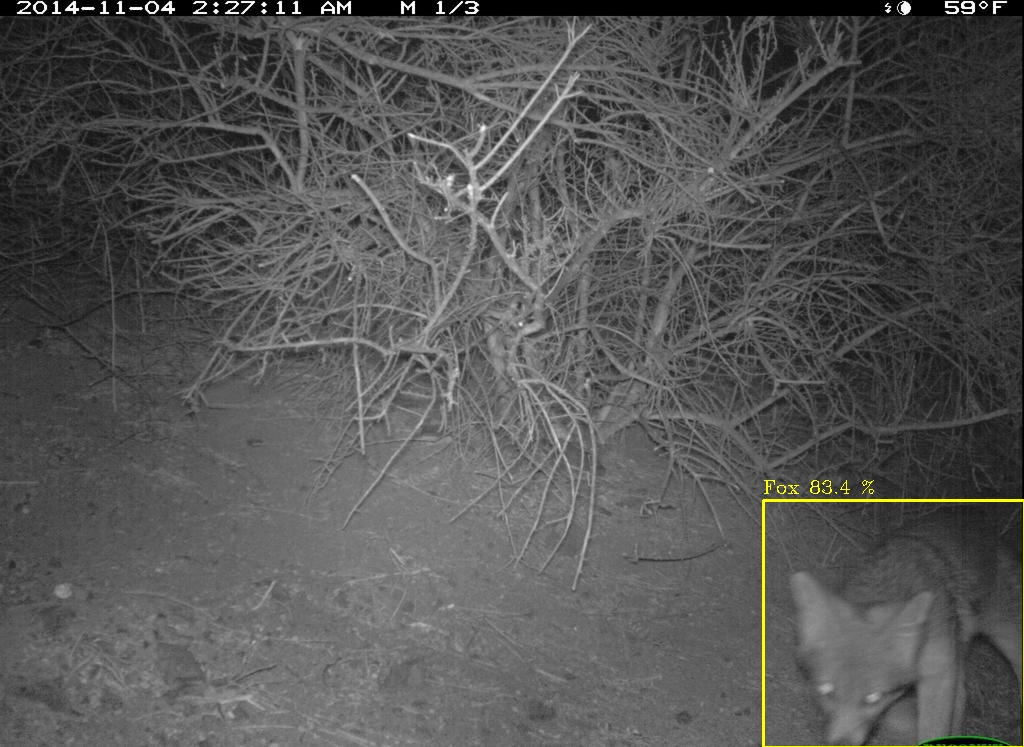
\includegraphics[width=\textwidth]{iWildCam/fox/cut/59df5ee1-23d2-11e8-a6a3-ec086b02610b_faster_rcnn_inception_v2_4000.jpg}
  \captionof{figure}{4000 Samples}
\end{minipage}
\begin{minipage}{0.333\textwidth}
  \centering
  \label{}
  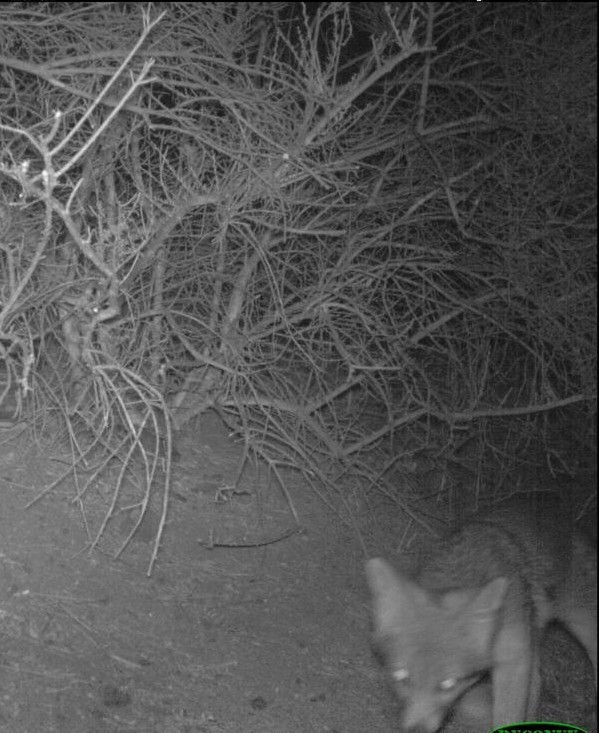
\includegraphics[width=\textwidth]{iWildCam/fox/cut/59df5ee1-23d2-11e8-a6a3-ec086b02610b_faster_rcnn_inception_v2_less_aug.jpg}
  \captionof{figure}{50\% Augment}
\end{minipage}

Bei der L2 Regulariesierung konnte für das iWildCam keine verbesserung festgestellt werden,
teilweise wurden die Bilder besser erkannt, teilweise schlechter, so dass im 
Mittel keine Verbesserung entstand.

Für die eigenen Bilder waren die Ergebnisse sogar schlechter.


\begin{minipage}{0.5\textwidth}
  \centering
  \label{}
  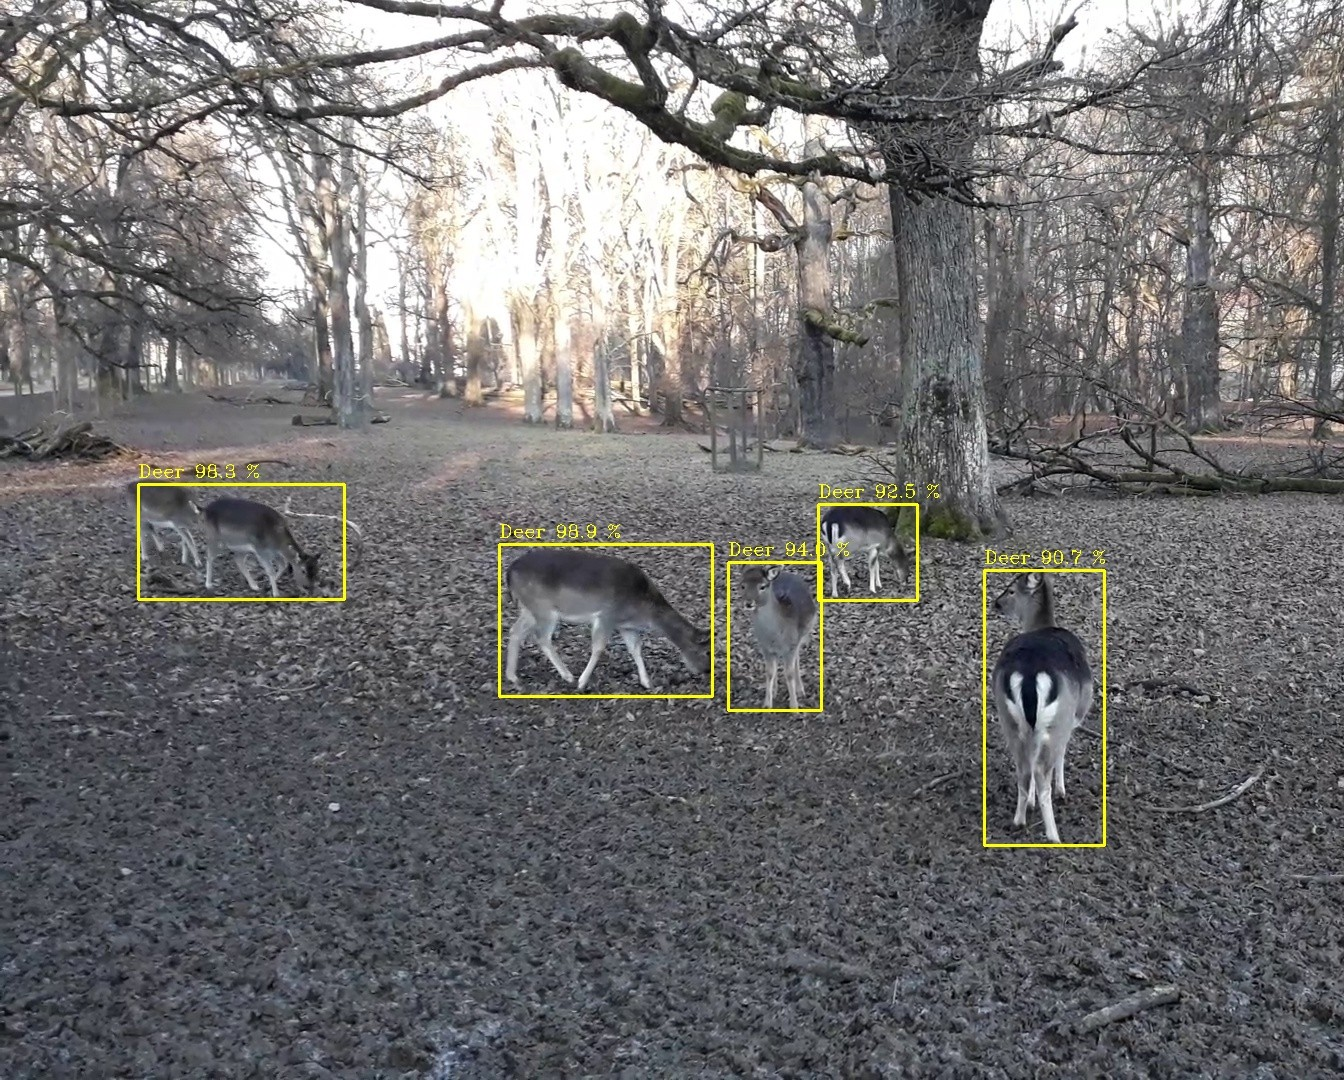
\includegraphics[width=0.95\textwidth]{eigene/20191229_145616_frame_20_faster_rcnn_inception_v2_3000.jpg}
  \captionof{figure}{}
\end{minipage}
\begin{minipage}{0.5\textwidth}
  \centering
  \label{}
  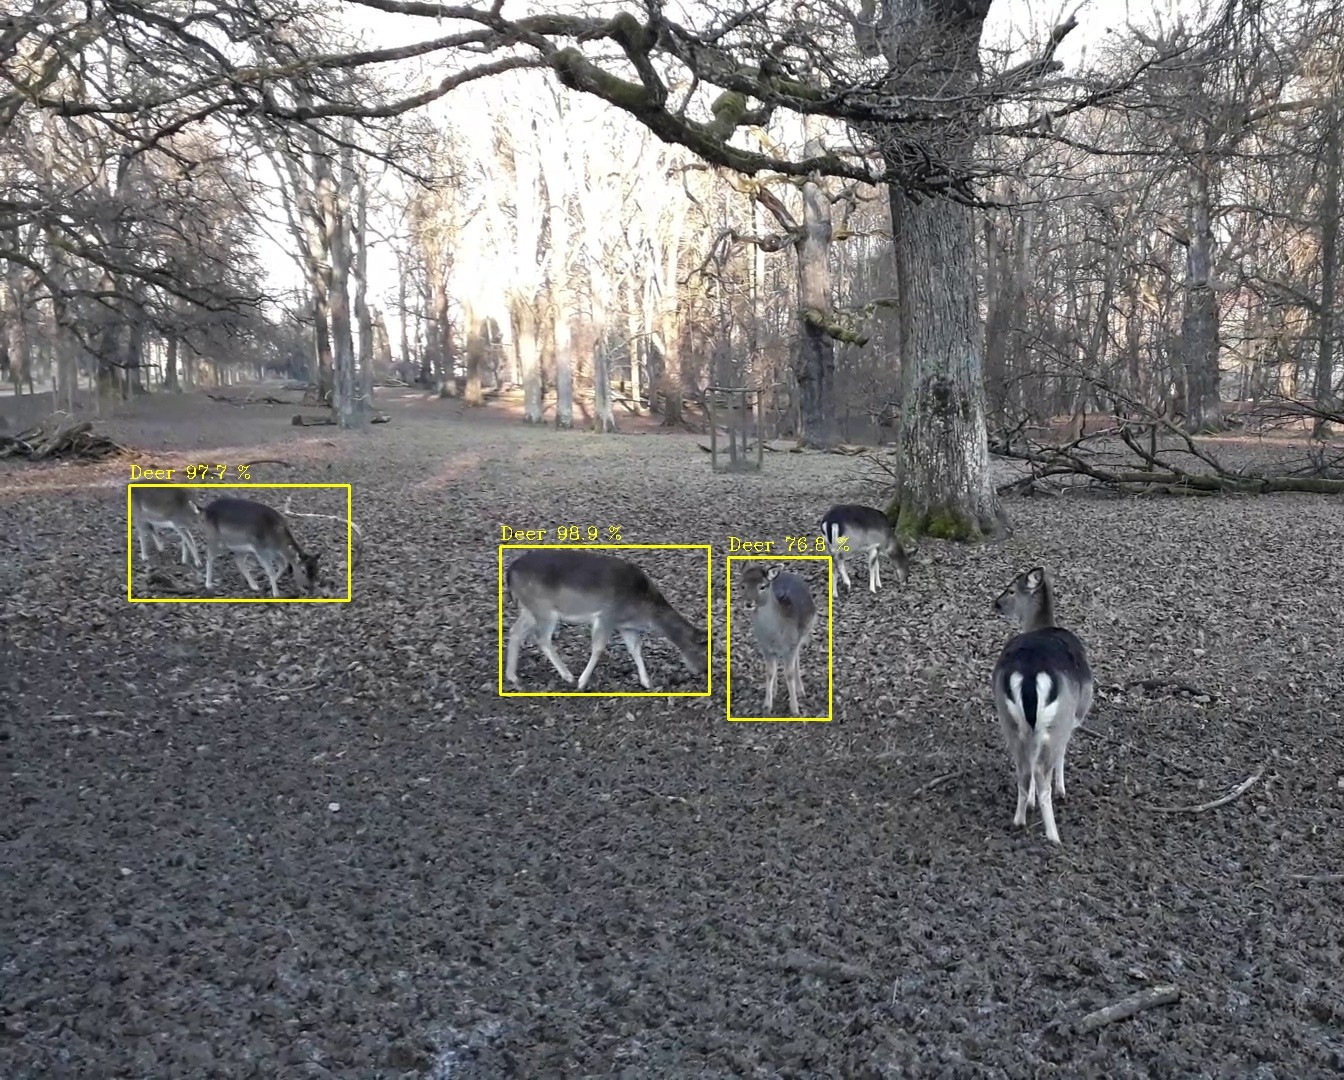
\includegraphics[width=0.95\textwidth]{eigene/20191229_145616_frame_20_faster_rcnn_inception_v2_l2.jpg}
  \captionof{figure}{}
\end{minipage}



Daraus lässt sich schließen das die Art/Qualität/Varianz der Daten 
den größeren einfluss auf das ergebniss haben und mit den Hyperparametern 
wenn überhaup



\subsection{Graustufen}
da kamerea graustufen bilder liefert, wurde getestet, ob ein 
training in graustufen bilder zu besseren erg führt, ... nicht so.



% \subsection{weitere tabellen}\label{subsec:regularisierung}

% \begin{table}[htb]
%     \centering
%     \label{tab:regularization}
%     \begin{tabular}{| l || c | c | c | c |} 
%         \hline
%         Regularisierung & $mAP_{orig}$ & $mAP_{handy}$ & $Loss_{orig}$ &  $Loss_{handy}$\\
%         \hline
%         Early Stopping (100k steps) & 0.6715 & 0.4265 & 0.6742 & 0.267\\
%         \hline
%         Augmentierung (200k steps) & 0.6914 & 0.4537 & 0.6738 & 0.2503\\ % hier noch verschiedene kombinationen von augmentierungen
%         \hline
%     \end{tabular}        
%     \caption{Regularization}
% \end{table}




% \subsection{Graustufen/Infrarot Bilder}\label{subsec:eval_gray}


% \begin{table}[htb]
%     \centering
%     \label{tab:eval_gray}
%     \begin{tabular}{| l | l || c | c |} 
%         \hline
%         Modell & Dataset & mAP & Loss\\
%         \hline
%         \multirow{2}{*}{rgb} & original & 0.6556 & 0.1451 \\
%         & handy & 0.4155 & 0.2389 \\
%         \hline
%         \multirow{2}{*}{gray 1 channel} & original & 0.5625 & 0.1716 \\
%         & handy & 0.3226 & 0.2747 \\
%         \hline
%         \multirow{2}{*}{gray 3 channel} & original & 0.664 & 0.1653 \\
%         & handy & 0.438 & 0.2492 \\
%         \hline
%     \end{tabular}        
%     \caption{Grayscale}
% \end{table}





\section{Inferenz zeit}

Neben der Genauigkeit ist die Ausführungszeit welche ein Model für die 
Inferenz benötigt, ein weiteres kriterium für die auswahl des Modells gewesen.
Je nach Anwendungsart muss diese in Echtzeit erfolgen oder nicht.

Ein Faktor von dem die Inferenzzeit abhängt ist die verwendeten Hardware
sowie Library. Für den Neural Compute Stick können dafür OpenCV oder 
OpenVino verwendetet werden, wobei mit OpenVino die möglichkeit 
zur asynchrone Inferenzausführung sowie mehreren Inferenz Requests wodurch 
sich die Inferenz zeit optimieren lässt.


Der zwiete Faktor wird durch die Komplexität des CNNs und der
zur Objekterkennung verwendeten Architektur bestimmt.

Üblicherweise sind Komplexere Modelle wie Faster R-CNN genauer jedoch 
auch langsamer.

Im folgenden soll daher zunächst die Asynchrone Inferenz näher 
erläutert werden und anschließen ein verfahren zur Untersuchung 
des Einfluss der Art der trainierten Modelle auf die Inferenz Zeit.

\subsection{Asychrone Inferenz}

Bei einem Synchronen inferenzablauf kann immer nur entweder inferiert oder 
die Daten vor- und nachverarbeitet werden. Da die inferenz jedoch auf dem 
Chip des NCS2 und nicht auf dem Pc oder Raspberry läuft, kann diese auch 
ungehindert parallel dazu ablaufen, was in OpenVino mit der Asychronen Api 
erreicht werden kann.

% inferenz
\begin{minipage}{0.5\textwidth}
  \centering
  \begin{algorithm}[H]
    \caption{Synchrone Inferenz}
    \begin{algorithmic}
    \WHILE{\TRUE}
        \STATE capture FRAME
        \STATE preprocess CURRENT InferRequest
        \STATE \textbf{start} CURRENT InferRequest
        \STATE \textbf{wait} for CURRENT InferRequest
        \STATE process CURRENT result
    \ENDWHILE
    \end{algorithmic}
  \end{algorithm}
\end{minipage}
\begin{minipage}{0.5\textwidth}
  \centering
  \begin{algorithm}[H]
    \caption{Asynchrone Inferenz}
    \begin{algorithmic}
    \WHILE{\TRUE}
        \STATE capture FRAME
        \STATE preprocess NEXT InferRequest
        \STATE \textbf{start} NEXT InferRequest
          \STATE \textbf{wait} for CURRENT InferRequest
          \STATE process CURRENT result
    \ENDWHILE
    \end{algorithmic}
  \end{algorithm}    
\end{minipage}

% https://docs.openvinotoolkit.org/2018_R5/_samples_object_detection_demo_ssd_async_README.html


\begin{figure}[htb]
    \centering
    \def\svgwidth{0.7\textwidth}
    \input{Bilder/synch_asynch.pdf_tex}
    \caption{Asynchron und mehrerere Inferenz Requests}
    \label{fig:async}
\end{figure}




\subsection{Vergleich der Modelle}

Mithilfe eines Python Scripts wurde nun die Inferenz für 100 Bilder 
ausgeführt und daraus die durchschnittliche Anzahl an Frames pro 
Sekunde berechnet (FPS).

Tabelle \ref{table:infertime} zeigt die ergebnisse für die 
Ausführung auf einem Raspberry Pi für die trainierten Modelle mit 
variierenden Inferenz Requests von einem bis vier.

\vspace{1cm}

\begin{table}[htb]
  \centering
  \label{table:infertime}
  \begin{tabular}{m{0.25\textwidth}|m{0.1\textwidth}<{\centering}|m{0.1\textwidth}<{\centering}|m{0.1\textwidth}<{\centering}|m{0.1\textwidth}<{\centering}}
  \hline
  \multirow{2}{*}{Model} & \multicolumn{4}{c}{Asynchronge Inferenz Requests} \\ \cline{2-5} 
                         & 1           & 2          & 3          & 4          \\ \hline\hline
  SSD MobilenetV2        & 19,5           & 35,2          & 40,6          & 40,3          \\
  SSD InceptionV2        & 15,6           & 27,7          & 31,1          & 31,7          \\
  Faster R-CNN Incept.   & 0,63           & 0,67          & 0,75          & 0,74          \\ \hline
  \end{tabular}
  \caption{Vergleich Inferenz Zeiten Modelle}
\end{table}

\vspace{1cm}

Insbesondere zwischen den Objeckt Detection Frameworks Faster R-CNN 
und SSD besteht ein froße Unterschied.
Möchte man die Inferenz für eine Echtzeitanwendung kommen nur SSD in Frage.
Desweiteren ist festzustellen, das eine erhöhung der Inferenz Requests 
nur bis 3 sinnvoll ist.


